\documentclass[tikz,border=3.14mm]{standalone}
\begin{document}
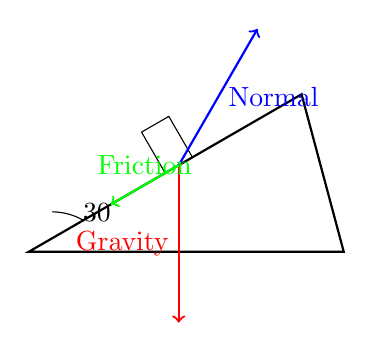
\begin{tikzpicture}[scale=2]

    % Angle of inclination
    \def\angle{30}
    
    % Plane
    \draw[thick] (0,0) -- ({2*cos(\angle)},{2*sin(\angle)}) -- (2,0) -- cycle;
    \draw[rotate=\angle] (1,0.3) rectangle (1.2, 0);
    
    % Forces
    \draw[->,thick,red] ({1.1*cos(\angle)}, {1.1*sin(\angle)}) -- ++(0, -1) node[midway,left] {Gravity};
    \draw[->,thick,blue] ({1.1*cos(\angle)},{1.1*sin(\angle)}) -- ++({90-\angle}:1) node[midway,right] {Normal};
    \draw[->,thick,green] ({1.1*cos(\angle)},{1.1*sin(\angle)}) -- ++({180+\angle}:0.5) node[midway,above] {Friction};
    
    % Angle notation
    \draw[thin] ({0.4*cos(\angle)}, {0.4*sin(\angle)}) arc({90-\angle}:90:0.4);
    \node at ({0.5*cos(\angle)}, {0.5*sin(\angle)}) {$\angle$};

\end{tikzpicture}
\end{document}